\documentclass[11pt]{article}
\usepackage{acl2015}
\usepackage{times}
\usepackage{url}
\usepackage{latexsym}
\usepackage{graphicx}
\usepackage{apacite}
% \usepackage{hyperref}
% \bibliographystyle{IEEEtran}
%\setlength\titlebox{5cm}

\title{BERT: Pre-training of Deep Bidirectional Transformers for Language Understanding}

\author{Dat Nguyen Duy \\
  {\tt 20520435} \\\And
  Khoa Tran Huu \\
  {\tt 20520222} \\\And
  Vu Huynh Hoang \\
  {\tt 20520864} \\\And
  Viet Le The \\
  {\tt 20520093} \\}

\date{}

\begin{document}
\maketitle
\begin{abstract}
\quad BERT, or Bidirectional Encoder Representations from Transformers, is a pre-trained language model in NLP that considers context from both the left and right sides of an input sequence, a departure from traditional NLP models that only consider context from one direction. BERT's bidirectional approach allows it to better understand the meaning of words in context, enabling it to handle more complex language relationships. This has made BERT highly effective in a wide range of NLP tasks, leading to new state-of-the-art results on benchmark datasets. BERT's pre-training and fine-tuning process, where the model is first pre-trained on a large corpus of text data and then fine-tuned on smaller task-specific datasets, makes it computationally efficient and allows for high accuracy with less data compared to training from scratch.
\end{abstract}

\section{Two main approaches}

\quad The two main approaches to applying pre-trained language models to downstream tasks are the feature-based approach and the fine-tuning approach.

The feature-based approach uses pre-trained models as a fixed feature extractor and feeds the representation into a separate task-specific model. This approach is computationally efficient and requires less training data but provides limited adaptability to the specific characteristics of the downstream task.

The fine-tuning approach involves updating the pre-trained model's weights to adapt to the specific characteristics of the downstream task, leading to better performance. However, it requires more computational resources and can lead to overfitting if the model is fine-tuned for too long, especially if the amount of training data for the downstream task is unsatisfactory.

The choice between these two approaches depends on the specific requirements of the downstream task and the available resources. The feature-based approach is suitable for tasks that are easier to interpretability and lack training data, while the fine-tuning approach is more suitable for tasks requiring high accuracy and sufficient training data.

\section{Introduction BERT}
\quad Based on Transformer Encoder in \cite{devlin2018bert}, a language representation model \textbf{BERT} which stands for \textbf{B}idirectional \textbf{E}ncoder \textbf{R}epresentations  from \textbf{T}ransformers publish in \cite{vaswani2017attention} 
has proven its robustness and flexibility by achieving state-of-the-art in many tasks in NLP. \\

There are two steps in the BERT framework: \textit{pre-training} and \textit{fine-tuning}. During the pre-training step, the model is trained on unlabeled data over different pre-training tasks. After the pre-training step, the model can understand the language. More specifically, we will obtain the representation of each token in the given input after finishing the pre-training step and use it to solve the downstream tasks by fine-tuning the step. For fine-tuning, parameters are fine-tuned using labeled data from the downstream tasks like ner, sequence labeling, …

A distinctive feature of BERT is its unified architecture across different tasks. There is minimal difference between the pre-trained architecture and the final downstream architecture.

\textbf{Model Architecture}\\

\begin{figure}[h]
    \centering
    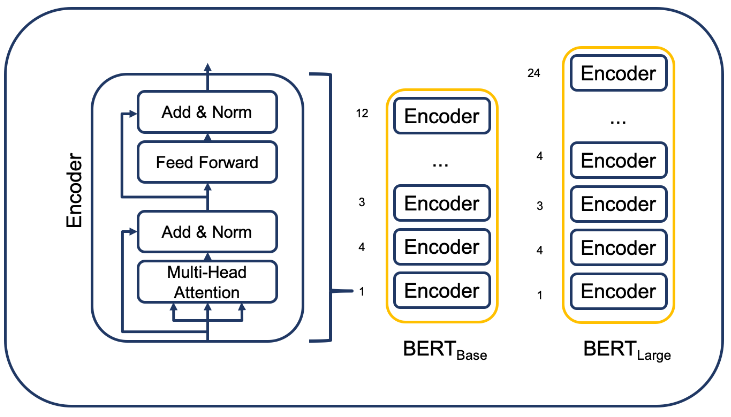
\includegraphics[width=0.47\textwidth]{BERT_model.png} \\
    \caption{BERT Encoder Stack} \cite{WinNT}
    \label{fig1}
\end{figure}


The architecture of BERT is Multi-layer bidirectional Transformer encoder, this is similar to the encoder part of the transformer architecture. Each encoder consists of two main parts: multi-head attention and Feed Forward Neural Network (FFNN). The data after embedding will go through the multi-head attention to learn the relationship between the words in the sentence, then go through the FFNN and be passed on to the next encoder block. In \cite{devlin2018bert}, there are two types of BERT's model size : 
\textbf{BERT}$_{BASE}$ (L=12, H=768, A=12, Total Parameters=110M) 
\textbf{BERT}$_{LARGE}$ (L=24, H=1024, A=16, Total Parameters=340M) where L is the number of layers, H is hidden size and A is the number of self-attention heads. \textbf{BERT}$_{BASE}$ is same model size as OpenAI GPT but uses \textbf{bidirectional self-attention}. \\

\textbf{Input Representations} To make BERT handle a variety of downstream tasks, always representing an input as a long sequence. A “sequence” refers to the input token sequence to BERT which may be a single sentence or two sentences packed together (e.g., h Question, Answer). \\

\begin{figure}[h]
    \centering
    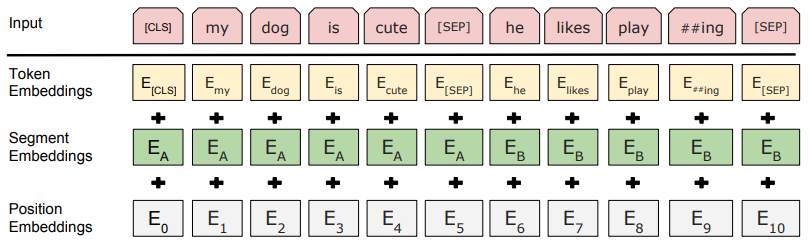
\includegraphics[width=0.47\textwidth]{BERT_input.png} \\
    \caption{Input Representation}
    \label{fig2}
\end{figure}


The first token of every sequence is always a special classification token ([CLS]). Specifically, each word in sequence was embeddings by using WordPiece embeddings. To separate the sentences in sequence. the authors use Segment embeddings by adding a Token ([SEP]) and a learned embedding EA, EB to know if each word belongs to sentence A or B. In previous research, it was found that Attention does not capture the word's position, so we also need Position embeddings. And we get input from BERT by summing each embedding together.


\section{Pretraining BERT}
\quad BERT was pre-training on two unsupervised tasks : Masked Language Modeling (Masked ML) and Next Sentence Prediction (NSP).

\begin{figure}
    \centering
    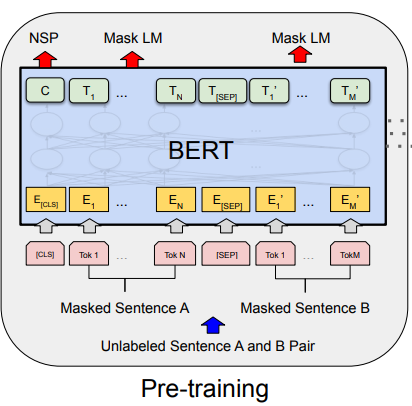
\includegraphics[width=0.47\textwidth]{pretraining.png} \\
    \caption{BERT pre-training}
    \label{fig:my_label}
\end{figure}

The first token at the output is the result of NSP task and remain is the result of Masked LM task.
\subsection{Masked LM}
\quad The deep bidirectional model is strictly more powerful than either left-to-right model or right-to-left model. But standard conditional language models can only be trained left-to-right or right-to-left. The reason is words can "see themselves" in a bidirectional context and the model could trivially predict the target word. To train a deep bidirectional representation, the authors mask 15$\%$ input tokens at random and then predict masked. \\

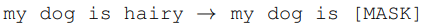
\includegraphics[width=0.47\textwidth]{MLM.png} \\

But there remain problems, training will be too expensive if we mask too little, if we mask too much we will not enough context to predict these masks, and finally is a mismatch between pre-training and fine-tuning because [MASK] token does not appear during fine-tuning. The solutions given is Don't always replace “masked” words with the actual [MASK] token. Instead: 
\begin{itemize}
 \item 80\% of the time: Replace with the [MASK] token\\
$\Rightarrow$ my dog is hairy → my dog is [MASK] 

 \item 10\% of the time: Replace with a random word\\
$\Rightarrow$ my dog is hairy → my dog is apple 

 \item 10\% of the time: Keep the word unchanged
$\Rightarrow$ my dog is hairy → my dog is hairy   
\end{itemize}

The advantage of this is
\begin{itemize}
    \item Encoder not know which words it will be asked to predict or which have been replaced by random words => forced to keep a distributional contextual representation of every input token.
    \item Random replacement only occurs for 1.5\% of all tokens (i.e., 10\% of 15\%), this does not seem to harm the model’s language understanding capability.
\end{itemize}


\subsection{NSP}
\label{sect:pdf}
\quad Many important downstream tasks are based on understanding the relationship between two sentences, which is not directly captured by language modeling. To help the model understand this, the authors pre-train BERT on binarized next sentence prediction task. \\

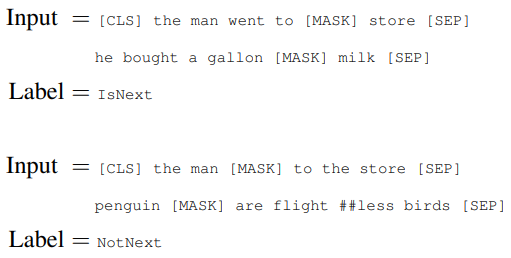
\includegraphics[width=0.47\textwidth]{NSP.png} \\

When choosing the sentences A and B for each pretraining example:
\begin{itemize}
    \item 50\% of the time B is the actual next sentence that follows A (labeled as IsNext)
    \item 50\% of the time it is a random sentence from the corpus (labeled as NotNext)
\end{itemize}

\textbf{Pre-training data} pre-training corpus that the authors are  using is BooksCorpus (800M words) (Zhu et al., 2015) and English Wikipedia (2,500M words, only the text passages and ignore lists, tables, and headers). More over, the authors was mention that need to
use a document-level corpus rather than sentence-level like Billion Word Benchmark to extract long contiguous sequences.

\section{Fine-tuning BERT}

\quad Fine-tuning is straightforward since the self attention in the Transformer allows BERT to implement many downstream tasks - 
whether are supervised-learning tasks that are improved based on pretrained models. For instance, We reuse the word representations that learned from pretrained models on large text sets into a training emotion analysis task on smaller text sets. Pre-training embedding help to improve the models.\cite{devlin2018bert}

\subsection{Special feature}

\begin{figure}[h]
	\centering
	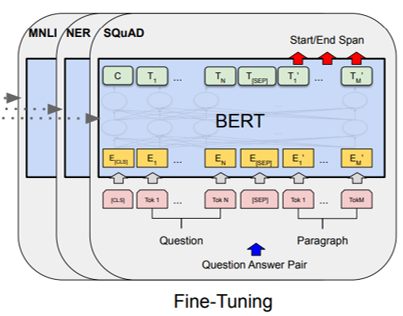
\includegraphics[width=0.5\textwidth]{fig0.png}
	\caption{Fine-tuning BERT architecture}
	\label{fig1}
\end{figure}

A special feature of BERT that previous embedding models have never had is that the training results can be fine-tuned. We will add to the model architecture an output layer to customize the training task.

During the fine-tuning process, all the parameters of the transfer learning layers will be fine-tuned.
\cite{devlin2018bert}

\subsection{Advantages of Fine-tuning}

\quad Quicker Development: The pre-trained BERT model weights already encode a lot of information about our language. As a result, it spends less time training our fine-tuned model. We have already trained the bottom layers of our network extensively and only tune them while using their output as features for our classification task. In fact, the researchers recommend only 2 to 4 epochs of training for fine-tuning BERT on a specific NLP task.

Less Data: Importantly, because of the pre-trained weights this model allows us to fine-tune our task on a much smaller dataset than would be required in a model that is built from scratch. A major disadvantage of NLP models built from scratch is that we often need a large dataset in order to train our network to better accuracy, meaning a lot of time and energy had to create dataset. By fine-tuning BERT, we can get away with training a model to good performance on a smaller amount of training data.

Better Results: Finally, this simple fine-tuning workflow (typically adding one fully-connected layer on top of BERT and training for a few epochs) was shown to achieve state of the art results with minimal task-specific adjustments for a wide variety of tasks: classification, language inference, semantic similarity, question answering, etc. Rather than implementing custom and sometimes-obscure architetures shown to work well on a specific task, simply fine-tuning BERT is shown to be a better alternative.\cite{mccormick2019bert}

\subsection{Fine-tuning steps}

\quad Step 1: Embedding all the tokens of the sentence pair by embedding vectors from the pretrain model. The embedding tokens include both [CLS] and [SEP] tokens to mark the beginning of the question and the space between the two sentences. These 2 tokens will be predicted in the output to determine the Start/End Spad parts of the output sentence.

Step 2: The vector embeddings are then fed into the multi-head attention architecture with multiple blocks of code (usually 6, 12, or 24 blocks depending on the BERT architecture). We obtain an output vector at the encoder.

Step 3: To predict the probability distribution for each word position in the decoder, at each time step we will pass to decoder the encoder's output vector and the decoder's embedding input vector to compute the encoder-decoder attention. Then project through the liner layer and softmax to obtain the probability distribution for the corresponding output at time step t.

Step 4: In the output of the transformer, we will fix the result of the Question so that it matches the Question in the input. The remaining positions will be the Start/End Span extension corresponding to the answer found from the input sentence
\cite{BERTmodel}
\subsection{Examples for Question-Answering task}

\quad Question: How many parameters does BERT-large have?

Reference: BERT-large is really big… it has 24 layers and an embedding size of 1024, for a total of 340M parameters! Altogether it is 1.34GB, so expect it to take a couple minutes to download to your Colab instance.
\begin{figure}[h]
	\centering
	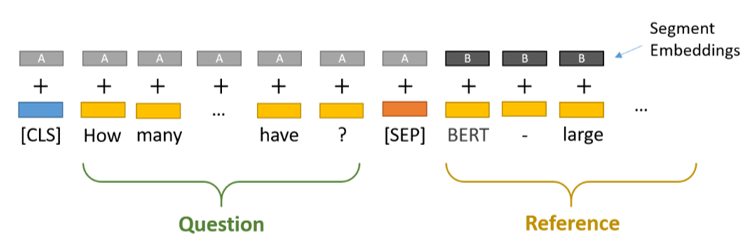
\includegraphics[width=0.5\textwidth]{fig1.png}
	\caption{Example in QA task}
	\label{fig1}
\end{figure}

Two types of text are separated by the special [SEP] token.

BERT also uses “Segment Embeddings” to differentiate the question from the reference text. These are simply two embeddings (for segments “A” and “B”) that BERT learned, and which it maps to the token embeddings before passing them into the input layer.
\cite{QAwithBERT}
\subsection{Example for Start and End Token Classifiers}

\quad BERT needs to highlight a span of text including the answer because this is simply predicting which token marks the start of the answer, and which token marks the end.

\begin{figure}[h]
	\centering
	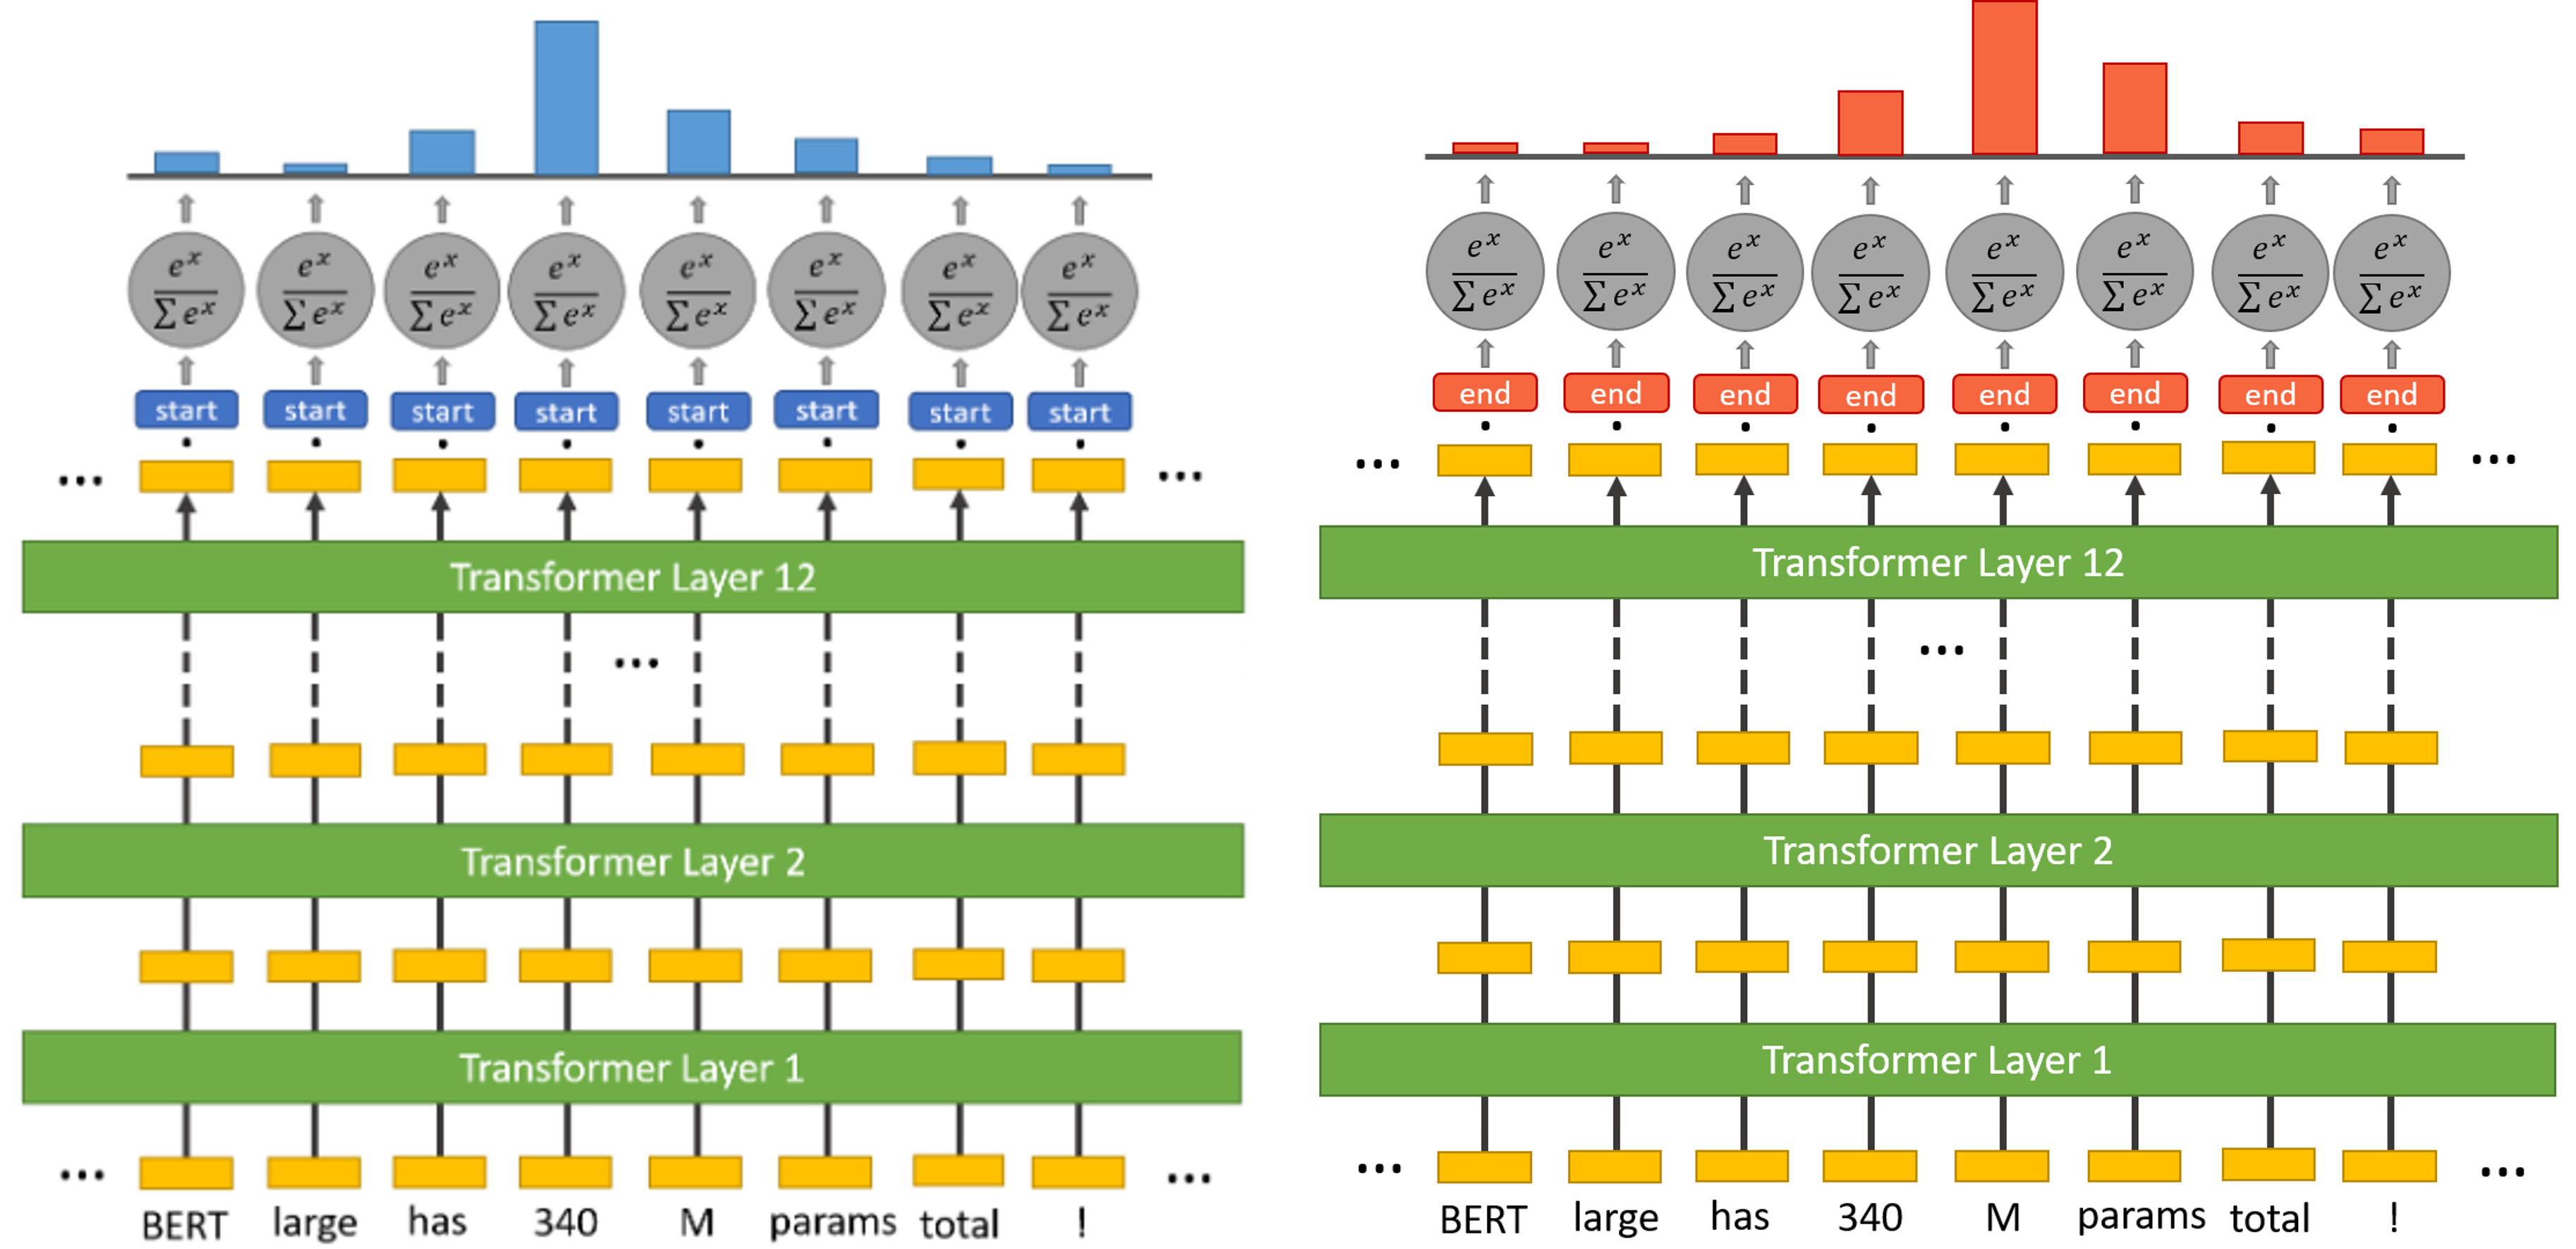
\includegraphics[width=0.5\textwidth]{fig2.png}
	\caption{Process for token classifying}
	\label{fig1}
\end{figure}

For every token in the text, we feed its final embedding into the start token classifier. The start token classifier only has a single set of weights (represented by the blue “start” rectangle in the above illustration) which it applies to every word.

After taking the dot product between the output embeddings and the ‘start’ weights, we apply the softmax activation to produce a probability distribution over all of the words. Whichever word has the highest probability of being the start token is the one that we pick.

We repeat this process for the end token–we have a separate weight vector this. \cite{QAwithBERT}

\section{Experiment}

\quad For experiment we used Bert for Binary Classification Task on Large Movie Review Dataset (aclImdb\_v1).

\subsection{ Large Movie Review Dataset}

\quad This is a dataset for binary sentiment classification containing substantially more data than previous benchmark datasets. We provide a set of 25,000 highly polar movie reviews for training and 25,000 for testing. 

This dataset has two classes, positive review, and negative review. Both the training set and the testing set have 50\% positive reviews and 50\% negative reviews.


In this task, we want the model can classify the review into two classes, positive or negative.

\subsection{ Using pretrained Bert model from Tensorflow Hub}

\quad TensorFlow Hub is a repository of trained machine learning models ready for fine-tuning and deployable anywhere. On Tensorflow Hub it has a lot of versions of pretrained Bert on a variety of different settings and each version has a preprocessing model comparable to it. Using pretrained models from TensorFlow Hub saves us a lot of time and resources.

\subsection{Fine-tune Bert model}

\begin{figure}[h]
	\centering
	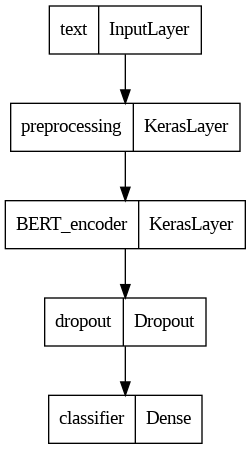
\includegraphics[width=0.2\textwidth]{b-cls-model.png}
	\caption{Layers of the model}
	\label{fig1}
\end{figure}

For fine-tuning phase, we implement a model which has 5 layers. First is the input layer, second is the preprocessing layer, third is the encoder layer which is the pretrained model, Fourth is the dropout layer to avoid overfitting, and the last layer is the output layer which has only one neuron for classification.

\subsection{Result}
\quad We using the Small Bert version for pretrained model, which have: the number of transformer layers is 2, the embedding length is 128, number of attention heads is 2.

We train the model in only 4 epochs and the accuracy on the training set is 0.799 and on the testing set is 0.779. The training time only takes about 7 minutes.

\begin{figure}[h]
	\centering
	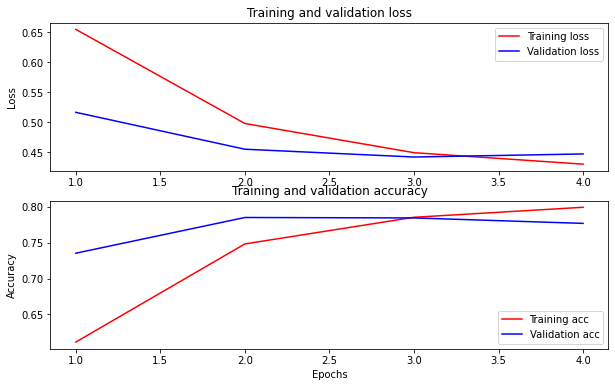
\includegraphics[width=0.5\textwidth]{graph.png}
	\caption{Train and validation loss seems to be converging well}
	\label{fig1}
\end{figure}

\bibliographystyle{apacite}
\bibliography{refs}
% \begin{thebibliography}{}

% \bibitem[\protect\citename{Aho and Ullman}1972]{Aho:72}
% Alfred~V. Aho and Jeffrey~D. Ullman.
% \newblock 1972.
% \newblock {\em The Theory of Parsing, Translation and Compiling}, volume~1.
% \newblock Prentice-{Hall}, Englewood Cliffs, NJ.

% \bibitem[\protect\citename{{American Psychological Association}}1983]{APA:83}
% {American Psychological Association}.
% \newblock 1983.
% \newblock {\em Publications Manual}.
% \newblock American Psychological Association, Washington, DC.

% \bibitem[\protect\citename{{Association for Computing Machinery}}1983]{ACM:83}
% {Association for Computing Machinery}.
% \newblock 1983.
% \newblock {\em Computing Reviews}, 24(11):503--512.

% \bibitem[\protect\citename{Chandra \bgroup et al.\egroup }1981]{Chandra:81}
% Ashok~K. Chandra, Dexter~C. Kozen, and Larry~J. Stockmeyer.
% \newblock 1981.
% \newblock Alternation.
% \newblock {\em Journal of the Association for Computing Machinery},
%   28(1):114--133.



% \bibitem[\protect\citename{Gusfield}1997]{Gusfield:97}
% Dan Gusfield.
% \newblock 1997.
% \newblock {\em Algorithms on Strings, Trees and Sequences}.
% \newblock Cambridge University Press, Cambridge, UK.

% \end{thebibliography}

\end{document}